\documentclass[12pt]{article}
%\usepackage[portuguese]{babel}
\usepackage[utf8]{inputenc}
\usepackage[usenames,dvipsnames]{color}
\usepackage{setspace}
\usepackage{amsmath}
\usepackage{amsfonts}
\usepackage{amssymb}
\usepackage{mathtools}
\usepackage[top=3cm, bottom=2cm, left=3cm, right=2cm]{geometry}
\usepackage{tikz}
\usepackage{indentfirst}
\usepackage{algorithm} % algorithms
\usepackage{algpseudocode} % algorithms
\usepackage{textcomp}
\title{Relatorio IC}

% packages added by Marcelo
%
\usepackage{lscape}    % for landscape pages
\usepackage{hyperref}  % to allow hyperlinks
\usepackage{booktabs}  % nicer table borders
\usepackage{subfigure} % add subfigures

\graphicspath{{./figures/}} 

\definecolor{myblue}{RGB}{80,80,160}
\definecolor{mygreen}{RGB}{80,160,80}
\setstretch{1.5}

\begin{document}

\begin{center}
{\Large Stochastic U-Curve Branch and Bound \\}
\bigskip
{\bf Student:} \href{mailto:estrela.gustavo.matos@gmail.com}{Gustavo Estrela de Matos} \\
        {\bf Advisor:} \href{mailto:ulisses@ece.tamu.edu}{Dr. Ulisses Braga-Neto}
\end{center}

\section{Input Generation}
To generate the input for the problem we created two functions. The first creates a vector of floating points that simulates the values of a chain of a boolean lattice that respects the U-Curve assumption; and the second one adds a random noise to the values of the vector.

\subsection{Chain Generation}
The algorithm receives three parameters: $n$, $max\_distance$ and $center$; and returns as output a vector that has values from $0$ to $1$ and respects the U-Curve assumption. The first parameter defines the size of the chain; the second represents the greatest possible difference between the values of neighbour nodes, which is a random value uniformily distributed between $0$ and $max\_distance$; and the last represents the index of the node with minimum value.

\begin{algorithm}[t]
\caption{U-Curve Input Creator}
\begin{algorithmic}[1]
\Procedure{GeneratePoints}{$n, max\_distance, center$}
    \State $points \gets \{0, ..., 0\}$
    \State $minimum \gets \frac{random ()}{2}$
    \State $points[center] \gets minimum$
    \State
    \For {$i \in \{0, ..., center - 1\}$}
        \State $points[i] \gets points[i + 1] + (1 - points[i + 1]) * random ()$
    \EndFor
    \For {$i \in \{center + 1, ..., n - 1\}$}
        \State $points[i] \gets points[i - 1] + (1 - points[i - 1]) * random ()$
    \EndFor
    \State
    \State $j \gets n * random ()$
    \State $plain_size \gets (n - j) * random ()$
    \For {$k \in \{1, ..., plain_size\}$} \Comment Creates a plain area in the chain
        \State $points[j + k] \gets points[j]$
    \EndFor
    \Return $points$
\EndProcedure
\end{algorithmic}
\end{algorithm}

\subsection{Noise}
The noise is applied to the vector created by $GeneratePoints$, by adding a value uniformily distributed in the interval 
$[-\alpha \frac{curve\_amplitude}{n}, \alpha \frac{curve\_amplitude}{n}]$, where $curve\_amplitude = max(v) - min (v)$ and $\alpha$ is a noise parameter.

\begin{figure}[H]
\caption{Example of a curve generated with $\alpha = 0$}
\centering
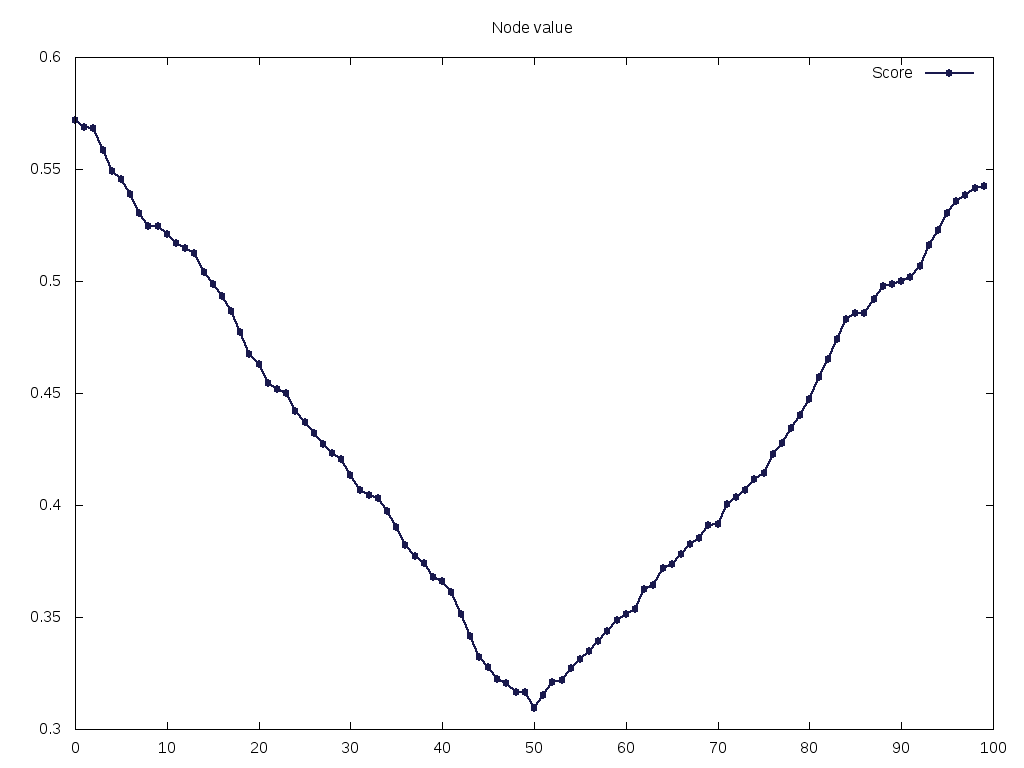
\includegraphics[scale=.5]{alpha_zero_curve}
\end{figure}

\begin{figure}[H]
\caption{Example of a curve generated with $\alpha = 1$}
\centering
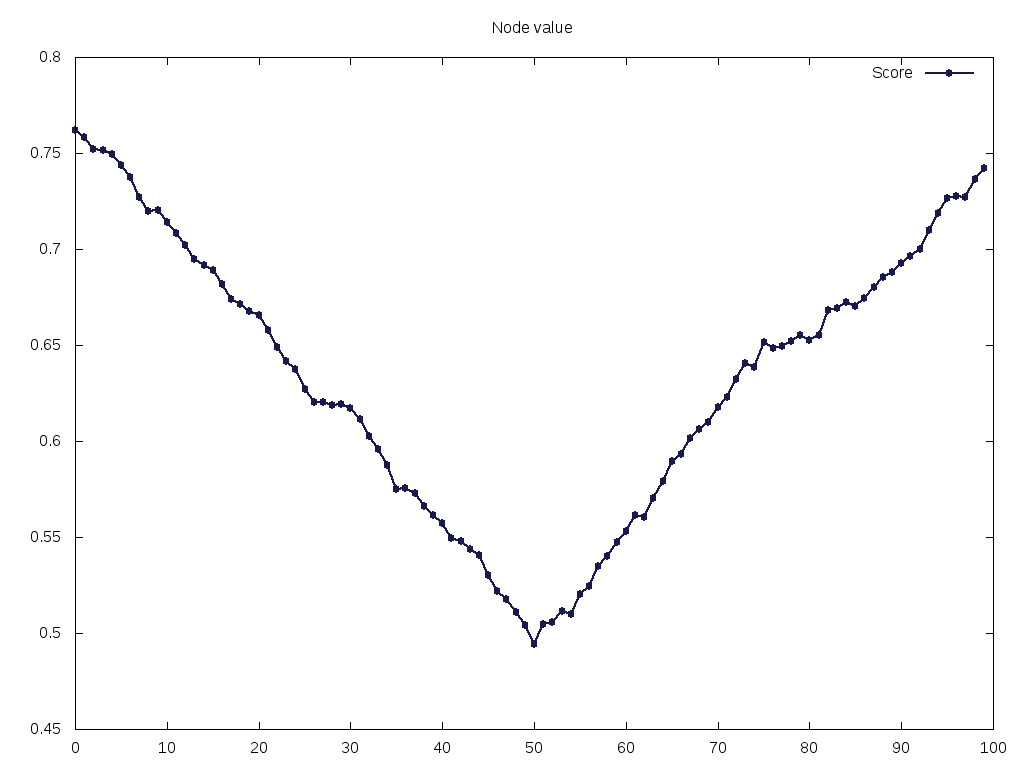
\includegraphics[scale=.5]{alpha_one_curve}
\end{figure}

\begin{figure}[H]
\caption{Example of a curve generated with $\alpha = 2$}
\centering
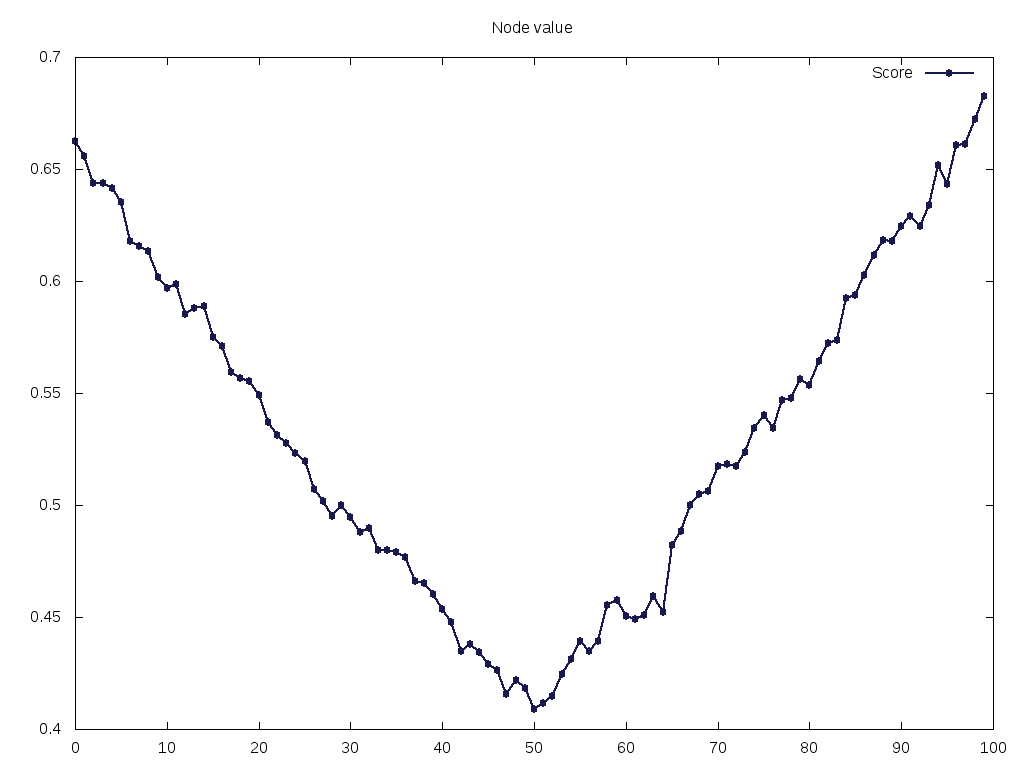
\includegraphics[scale=.5]{alpha_two_curve}
\end{figure}

\newpage
\section{Bisection Algorithms}
\end{document}

